\chapter{Experiments}\label{experiments}

\section{Overall Aims}
\label{sec: Overall Aims}
The aim of the broader experimentation was to see how the agents behave in an environment in which they all live and interact together and to see what changes when disruptive agents are introduced.
Several variables were considered for each experiment, each of which are discussed in the following sections.
The main dependent variable that will be considered is the death rate which determines the system stability. We also sought to observe the dependency on self-organisation to achieve stability and the effect of treaties and cooperation on self-organisation. Therefore, another important dependent variable that was measured was the number of treaties accepted and rejected by agents.

\section{Disruptive Agents}
\label{sec: Disruptive Agents}
The disruptive agents to be used in the following experiments were a random agent and a selfish agent. They have the following behaviours:
\begin{itemize}
    \item Random Agent: takes random amounts of food every tick.
    \item Selfish Agent: takes food every tick such that it always attempts to stay at maximum health.
\end{itemize}

\section{Stability}
\label{sec: Stability}
Before the effect of the parameters on stability can be measured, we must first define system stability. Stability is defined by Ashby as: “In all cases, the stable system is characterised by the fact that after a displacement we can assign some bound to the subsequent movement of the representative (equilibrium) point.”\cite{Ashby1960}
The features of a system's stability as given by \cite{Ashby1960} are as follows:
\begin{itemize}
    \item Stability refers to some aspect of a system, not the system itself.
    \item A stable system is brought back to a state of equilibrium when it is displaced.
    \item Stability is a property of the whole system.
    \item Presence of stability implies some coordination of action of the parts.
\end{itemize}
 
In the case of the tower as a system, the death rate is considered to be the equilibrium point and the displacement being the addition of agents to the tower since, before the introduction of the agents, there is no movement in any of the parameters of the system. The equilibrium point being a death rate of zero. 

The tower can therefore be considered stable if:
\begin{itemize}
    \item The death rate reaches zero, and
    \item The death rate stays at zero for at least one reshuffle period, and
    \item The death rate stays at zero until the end of the simulation.
\end{itemize}
 
This definition of tower stability also satisfies all four requirements mentioned above and by Ashby.

\section{Experiment 1}
\label{sec: Experiment 1}
\subsection{Aims}
\label{subsec: E1-Aims}
The aim of this experiment is to observe the impact of the addition of disruptive agents on the tower. 
We keep an equal number of each team’s agents in the tower. Selfish agents and random agents are then added. The food per agent on the platform (food scarcity) is also varied. This allows us to observe the effect of food scarcity on stability and the effect of the addition of these disruptive agents on tower stability. We expect as food becomes more scarce and as more disruptive agents are added, that the total number of deaths will increase and that stability will be more difficult to achieve.

In this experiment the tower being used is highly heterogeneous, with three of each team agent type being added to it. Three random agents, three selfish agents or three of both, or none of either will then be added to to the tower.
\subsection{Results and Discussion}
\label{subsec: E1-Results and Discussion}

\begin{figure}[H] %Treaties Rejected As Food Scarcity Decreases
    \centering
    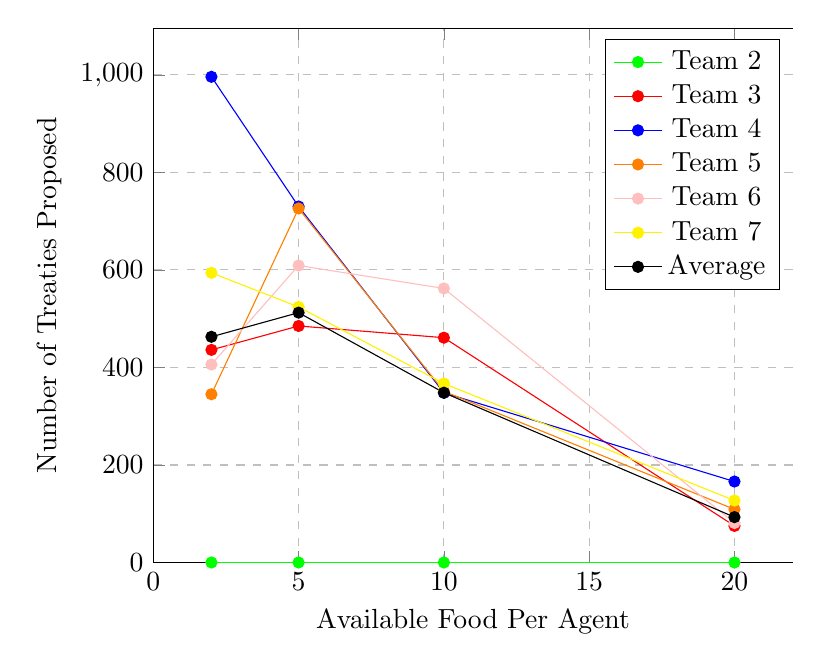
\begin{tikzpicture}
        \begin{axis}[
            width=0.8\textwidth,
            axis y line*=left,
            ymin=0,
            xmin=0,
            xlabel=Available Food Per Agent,
            ylabel=Number of Treaties Proposed,
            ymajorgrids=true,
            xmajorgrids=true,
            grid style=dashed,
        ]
        \addplot[mark=*,green]
            coordinates{
                (2, 0)
                (5, 0)
                (10, 0)
                (20, 0)
            }; \label{leg:team2-scarcity}
        \addplot[mark=*,red]
            coordinates{
                (2, 436)
                (5, 485)
                (10, 461)
                (20, 75)
            }; \label{leg:team3-scarcity}
        \addplot[mark=*,blue]
            coordinates{
                (2, 996)
                (5, 730)
                (10, 348)
                (20, 166)
            }; \label{leg:team4-scarcity}
        \addplot[mark=*,orange]
            coordinates{
                (2, 345)
                (5, 726)
                (10, 351)
                (20, 109)
            }; \label{leg:team5-scarcity}
        \addplot[mark=*,pink]
            coordinates{
                (2, 406)
                (5, 609)
                (10, 562)
                (20, 81)
            }; \label{leg:team6-scarcity}
        \addplot[mark=*,yellow]
            coordinates{
                (2, 594)
                (5, 524)
                (10, 367)
                (20, 127)
            }; \label{leg:team7-scarcity}
        \addplot[mark=*,black]
            coordinates{
                (2, 462.83)
                (5, 512.33)
                (10, 348.17)
                (20, 93)
            }; \label{leg:average-scarcity}
        \addlegendimage{/pgfplots/refstyle=leg:team2-scarcity}\addlegendentry{Team 2}
        \addlegendimage{/pgfplots/refstyle=leg:team3-scarcity}\addlegendentry{Team 3}
        \addlegendimage{/pgfplots/refstyle=leg:team4-scarcity}\addlegendentry{Team 4}
        \addlegendimage{/pgfplots/refstyle=leg:team5-scarcity}\addlegendentry{Team 5}
        \addlegendimage{/pgfplots/refstyle=leg:team6-scarcity}\addlegendentry{Team 6}
        \addlegendimage{/pgfplots/refstyle=leg:team7-scarcity}\addlegendentry{Team 7}
        \addlegendimage{/pgfplots/refstyle=leg:average-scarcity}\addlegendentry{Average}
        \end{axis}
        \end{tikzpicture}
    \caption{Number of Treaties Proposed as Food Scarcity Decreases}
    \label{fig:team1-robustness-food-scarcity}
\end{figure}

\Cref{team1-robustness-food-scarcity} illustrates the change in the frequency of treaty proposals as the constraints from the economy of scarcity are levied. The experiment enforces that there is 100 food initially available on the platform, with the number of agents parameterised to allow for an average amount of food per agent. This simulation lasts 400 days.

The general tendency for this system is that, as the availability of food rises (and hence the economy of scarcity becomes less constrictive), the rate of treaty proposals decreases. We propose that this experiment yields insight into the importance of treaties, demonstrating that agents in general rely heavily on treaty formation to self-organise when survivability is hindered by a lack of resources. Contrarily, as the food availability reaches an abundance, we see the rate of treaty proposals tend to 0, suggesting that agents are able to survive without the need for treaties as they offer little utility.

We also assert that this graph details the implied benefit of signing treaties: agents seem to value treaties as a means to fairer food distribution, wherein signing facilitates them receiving a greater proportion of food than they would otherwise receive without a treaty.

\begin{figure}[H] %Deaths As Food Scarcity Decreases with different agent combos added
    \centering
    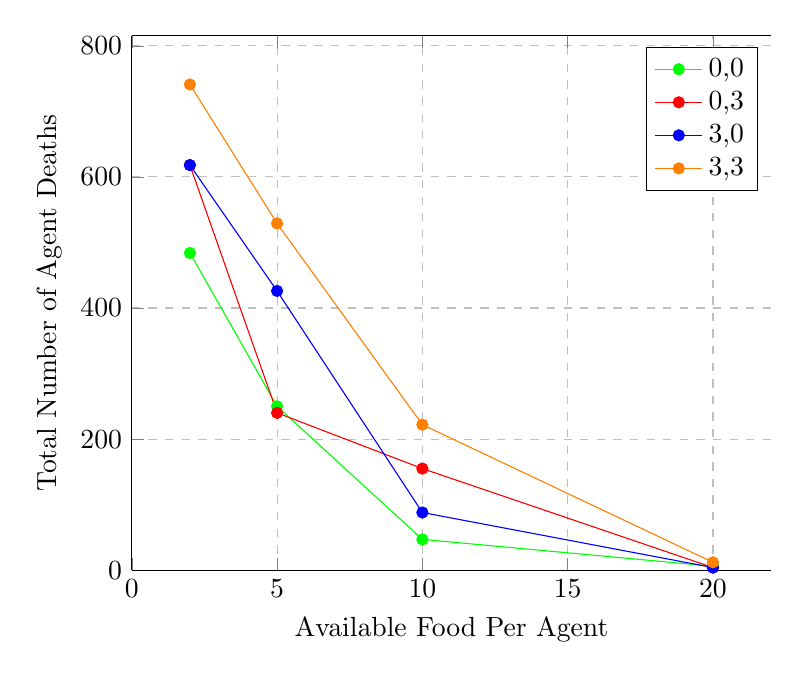
\begin{tikzpicture}
        \begin{axis}[
            width=0.8\textwidth,
            axis y line*=left,
            ymin=0,
            xmin=0,
            xlabel=Available Food Per Agent,
            ylabel=Total Number of Agent Deaths,
            ymajorgrids=true,
            xmajorgrids=true,
            grid style=dashed,
        ]
        \addplot[mark=*,green]
            coordinates{
                (2, 484)
                (5, 250)
                (10, 47)
                (20, 6)
            }; \label{leg:scarcity00}
        \addplot[mark=*,red]
            coordinates{
                (2, 618)
                (5, 240)
                (10, 155)
                (20, 4)
            }; \label{leg:scarcity03}
        \addplot[mark=*,blue]
            coordinates{
                (2, 618)
                (5, 426)
                (10, 88)
                (20, 4)
            }; \label{leg:scarcity30}
        \addplot[mark=*,orange]
            coordinates{
                (2, 741)
                (5, 529)
                (10, 222)
                (20, 12)
            }; \label{leg:scarcity33}
        \addlegendimage{/pgfplots/refstyle=leg:scarcity00}\addlegendentry{0,0}
        \addlegendimage{/pgfplots/refstyle=leg:scarcity03}\addlegendentry{0,3}
        \addlegendimage{/pgfplots/refstyle=leg:scarcity30}\addlegendentry{3,0}
        \addlegendimage{/pgfplots/refstyle=leg:scarcity33}\addlegendentry{3,3}
        \end{axis}
        \end{tikzpicture}
    \caption{The total number of deaths in systems with different combinations of selfish and random agents added as food per agent increases. The number of each disruptive agent added to each system is show in the legend in the form (number of selfish agents, number of random agents)}
    \label{fig:team1-robustness-food-scarcity-disruptive-agents}
\end{figure}

\Cref{team1-robustness-food-scarcity-disruptive-agents} shows how the number of deaths is affected when different disruptive agents are added. It shows that, as expected, the number of deaths is higher when disruptive agents are present. However, the effect of selfish agents and random agents seems to be similar which suggests that it it not the amount of food being taken by the agents that is disruptive, rather it is the fact that they do not communicate that causes a higher death rate. This makes it harder to self-organise and makes it much harder to survive in the tower. 
By making it harder to survive in the tower, the chances of reaching a stable system are also decreased when disruptive agents are added. The only system to stabilise with ten food per agent was the one with no disruptive agents, all systems were stable with a tower of 20 food per agent.
\subsection{Conclusion}
\label{subsec: E1-Conclusion}
This experiment shows the importance of treaties and communication for the survival of the agents in the tower and shows that self-organisation is a key factor in the ability of the tower to reach a stable state.

\section{Experiment 2}
\label{subsec: Experiment 2}
\subsection{Aims}
\label{subsec: E2-Aims}
The aim of this experiment is to vary the number of ticks per floor and reshuffle period and observe the effects of this on tower stability and ability to self-organise.
\subsection{Results and Discussion}
\label{subsec: E2-Results and Discussion}

\begin{figure}[H] %Number of Deaths As Shuffle Period Decreases
    \centering
    \begin{minipage}{0.8\textwidth}
        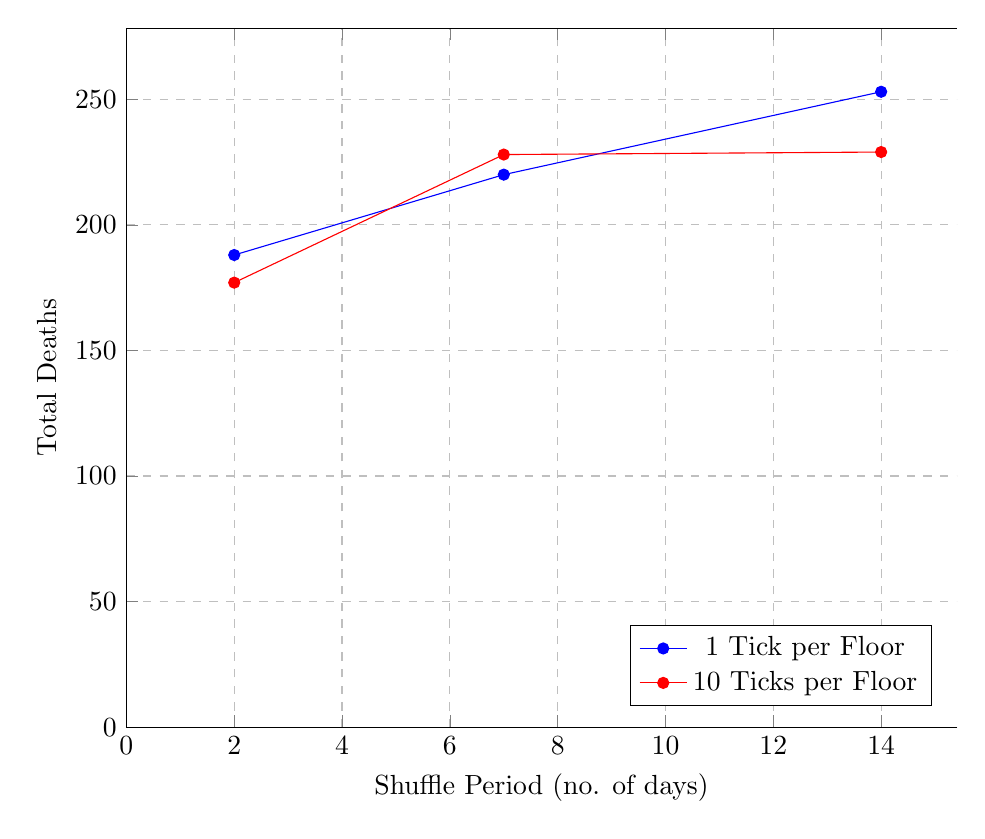
\begin{tikzpicture}
            \begin{axis}[
                width=\textwidth,
                axis y line*=left,
                ymin=0,
                xmin=0,
                xlabel=Shuffle Period (no. of days),
                ylabel=Total Deaths,
                ymajorgrids=true,
                xmajorgrids=true,
                grid style=dashed,
                legend pos=south east
            ]
            \addplot[mark=*,blue]
                coordinates{
                    (14, 253)
                    (7, 220)
                    (2, 188)
                }; \label{leg:reshuffle-ticks-per-floor1}
            \addplot[mark=*,red]
                coordinates{
                    (14, 229)
                    (7, 228)
                    (2, 177)
                }; \label{leg:reshuffle-ticks-per-floor10}
            \addlegendimage{/pgfplots/refstyle=leg:reshuffle-ticks-per-floor1}
            \addlegendentry{1 Tick per Floor}
            \addlegendimage{/pgfplots/refstyle=leg:reshuffle-ticks-per-floor10}\addlegendentry{10 Ticks per Floor}
            \end{axis}
        \end{tikzpicture}
    \end{minipage}
    \caption{Total Deaths in the Tower as Reshuffle Period Increases}
    \label{fig:Number-of-Deaths-As-Shuffle-Period-Decreases}
\end{figure}

\Cref{fig:Number-of-Deaths-As-Shuffle-Period-Decreases} investigates the correlation between the global deaths in the tower and the time between reshuffle periods.

A clear positive correlation emerges in this experiment, strongly supporting that the longer the periods between reshuffling, the more total deaths there are in the tower.

Similarly, we can see that the frequency of interaction (defined by the number of ticks per floor) has no overall impact on the death rate, suggesting that the quantity of communication is not the key factor in explaining these results. Furthermore, through propagation of treaties, we assert that the social network can still be formed effectively, even with increasing reshuffle periods.

For this reason, we propose that it is the rapid redistribution of agents throughout the tower, allowing them to experience varying levels of available food, that accounts for the disparity in survival rate: if an agent is consistently assigned to a low floor, they have a low chance of being satisficed if all agents act individually. Having a rapid reshuffle period results in a higher probability of reaching a higher floor, allowing for the agent to replenish its health. 

The average age of agents, denoted by \Cref{Average-Age-as-Shuffle-Period-Decreases}, can be seen to follow the inverse trend to death rates, as expected. This indicates that the longer the reshuffle period the lower the average age of an agent upon death. 
\begin{figure}[H] %Average Age As Shuffle Period Decreases
    \centering
    \begin{minipage}{0.8\textwidth}
        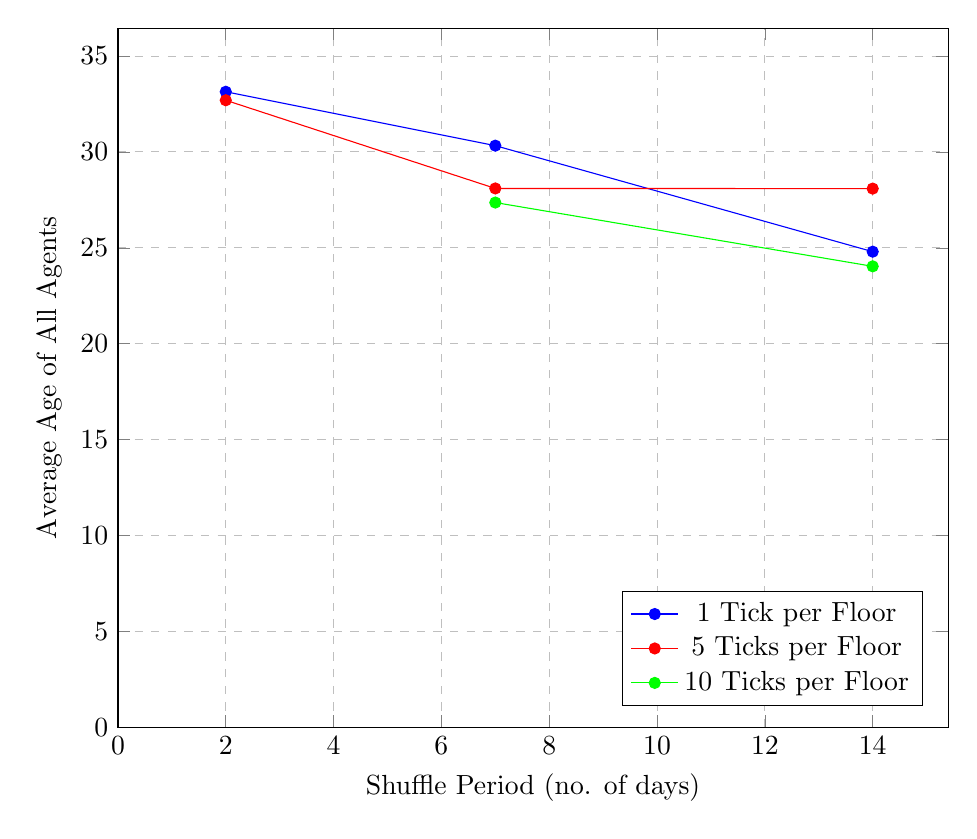
\begin{tikzpicture}
            \begin{axis}[
                width=\textwidth,
                ymin=0,
                xmin=0,
                xlabel=Shuffle Period (no. of days),
                ylabel=Average Age of All Agents,
                ymajorgrids=true,
                xmajorgrids=true,
                grid style=dashed,
                legend pos=south east
            ]
            \addplot[mark=*,blue]
                coordinates{
                    (14, 24.798)
                    (7, 30.327)
                    (2, 33.138)
                }; \label{leg:reshuffle-ticks-per-floor1}
            \addplot[mark=*,red]
                coordinates{
                    (14, 28.087)
                    (7, 28.096)
                    (2, 32.695)
                }; \label{leg:reshuffle-ticks-per-floor10}
            \addplot[mark=*,green]
                coordinates{
                    (14, 24.034)
                    (7, 27.36)
                }; \label{leg:reshuffle-ticks-per-floor5}
            \addlegendimage{/pgfplots/refstyle=leg:reshuffle-ticks-per-floor1}
            \addlegendentry{1 Tick per Floor}
            \addlegendimage{/pgfplots/refstyle=leg:reshuffle-ticks-per-floor5}
            \addlegendentry{5 Ticks per Floor}
            \addlegendimage{/pgfplots/refstyle=leg:reshuffle-ticks-per-floor10}\addlegendentry{10 Ticks per Floor}
            \end{axis}
        \end{tikzpicture}
    \end{minipage}
    \caption{Average Age in the Tower as Reshuffle Period Increases}
    \label{fig:Average-Age-as-Shuffle-Period-Decreases}
\end{figure}

\Cref{fig:Total-Accepted-Treaties-As-Shuffle-Period-Decreases} and \Cref{fig:Total-Rejected-Treaties-As-Shuffle-Period-Decreases} show that significant numbers of treaties are being exchanged at all reshuffle periods, demonstrating that a social network is being formed. However, as the reshuffle period decreases the total number of treaties proposed also decreases. This is as expected since, if agents have the same neighbours for longer periods of time, they need to exchange fewer new treaties, given that each proposed treaty will be agreed upon by neighbours for longer and so neighbours will not need to send each other new treaties. 

\begin{figure}[H] %Total Accepted Treaties As Shuffle Period Decreases
    \centering
    \begin{minipage}{0.8\textwidth}
        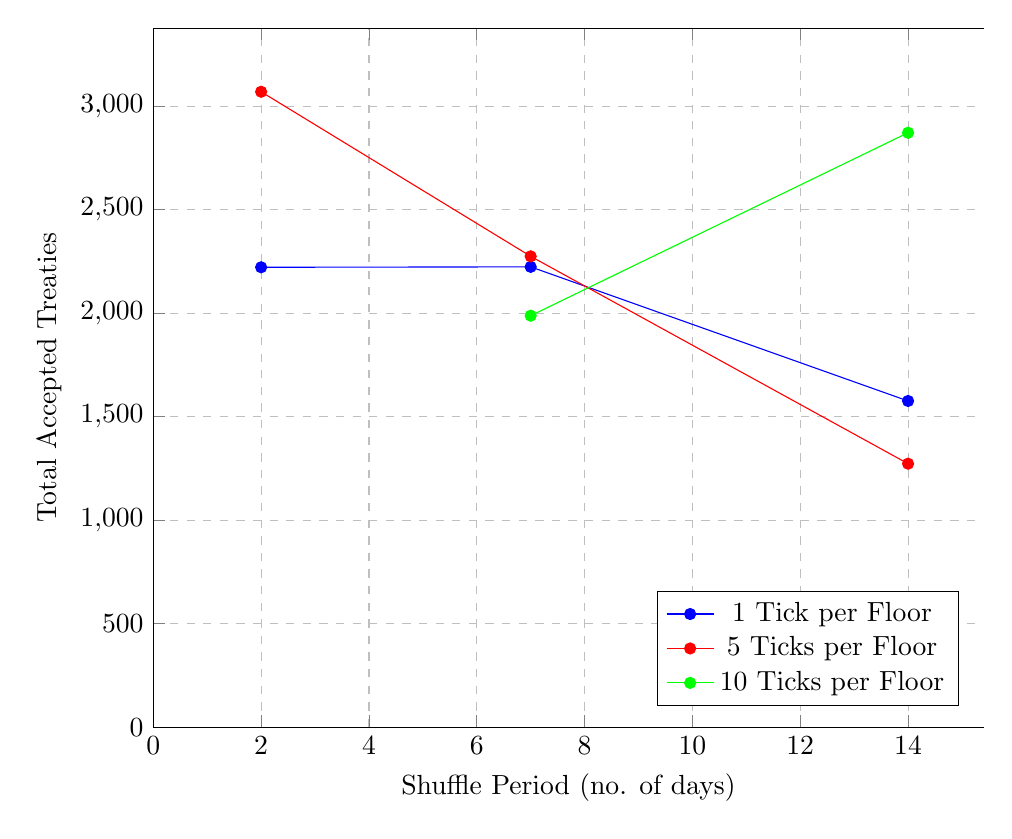
\begin{tikzpicture}
            \begin{axis}[
                width=\textwidth,
                axis y line*=left,
                ymin=0,
                xmin=0,
                xlabel=Shuffle Period (no. of days),
                ylabel=Total Accepted Treaties,
                ymajorgrids=true,
                xmajorgrids=true,
                grid style=dashed,
                legend pos=south east
            ]
            \addplot[mark=*,blue]
                coordinates{
                    (14, 1576)
                    (7, 2224)
                    (2, 2222)
                }; \label{leg:reshuffle-ticks-per-floor1}
            \addplot[mark=*,red]
                coordinates{
                    (14, 1273)
                    (7, 2275)
                    (2, 3070)
                }; \label{leg:reshuffle-ticks-per-floor10}
            \addplot[mark=*,green]
                coordinates{
                    (14, 2872)
                    (7, 1988)
                }; \label{leg:reshuffle-ticks-per-floor5}
            \addlegendimage{/pgfplots/refstyle=leg:reshuffle-ticks-per-floor1}
            \addlegendentry{1 Tick per Floor}
            \addlegendimage{/pgfplots/refstyle=leg:reshuffle-ticks-per-floor5}
            \addlegendentry{5 Ticks per Floor}
            \addlegendimage{/pgfplots/refstyle=leg:reshuffle-ticks-per-floor10}\addlegendentry{10 Ticks per Floor}
            \end{axis}
        \end{tikzpicture}
    \end{minipage}
    \caption{Total Accepted Treaties As Shuffle Period Decreases}
    \label{fig:Total-Accepted-Treaties-As-Shuffle-Period-Decreases}
\end{figure}

\begin{figure}[H] %Total Rejected Treaties As Shuffle Period Decreases
    \centering
    \begin{minipage}{0.8\textwidth}
        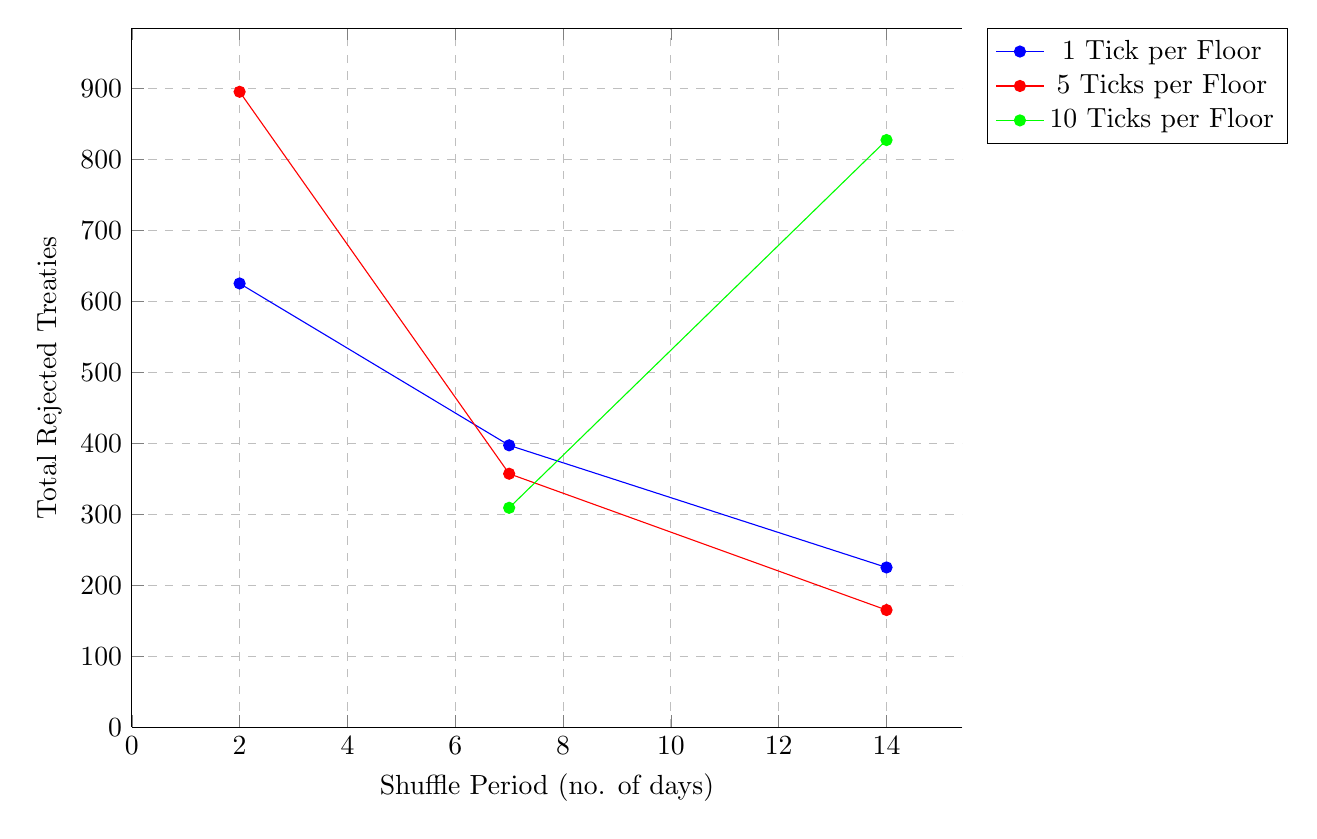
\begin{tikzpicture}
            \begin{axis}[
                width=\textwidth,
                axis y line*=left,
                ymin=0,
                xmin=0,
                xlabel=Shuffle Period (no. of days),
                ylabel=Total Rejected Treaties,
                ymajorgrids=true,
                xmajorgrids=true,
                grid style=dashed,
                legend pos=outer north east
            ]
            \addplot[mark=*,blue]
                coordinates{
                    (14, 225)
                    (7, 397)
                    (2, 625)
                }; \label{leg:reshuffle-ticks-per-floor1}
            \addplot[mark=*,red]
                coordinates{
                    (14, 165)
                    (7, 357)
                    (2, 895)
                }; \label{leg:reshuffle-ticks-per-floor10}
            \addplot[mark=*,green]
                coordinates{
                    (14, 827)
                    (7, 309)
                }; \label{leg:reshuffle-ticks-per-floor5}
            \addlegendimage{/pgfplots/refstyle=leg:reshuffle-ticks-per-floor1}
            \addlegendentry{1 Tick per Floor}
            \addlegendimage{/pgfplots/refstyle=leg:reshuffle-ticks-per-floor5}
            \addlegendentry{5 Ticks per Floor}
            \addlegendimage{/pgfplots/refstyle=leg:reshuffle-ticks-per-floor10}\addlegendentry{10 Ticks per Floor}
            \end{axis}
        \end{tikzpicture}
    \end{minipage}
    \caption{Total Rejected Treaties As Shuffle Period Decreases}
    \label{fig:Total-Rejected-Treaties-As-Shuffle-Period-Decreases}
\end{figure}

\subsection{Conclusion}
\label{subsec: E2-Conclusion}
The change in reshuffle period and number of ticks per floor does not have a significant impact on the ability of the agents to self-organise. However, increasing the reshuffle period does increase the number of deaths and so would make reaching stability more difficult.


